\section{Architecture of the whole system}
The architecture of the system is shown in figure \ref{fig:Architecture}. The system in it's whole is running on the student's phone. The main components are the presentation layer and game engine, where the purpose has been to make the game engine very generic and loosely coupled from the presentation layer. By replacing the presentation layer, the Game Engine can be implemented in a web application or using Google Assistant which uses voice to interact. 

We'll briefly dicuss the the architecture of the system in the following subsections, before we'll give a more thorough expalantion.

\begin{figure}[h!]
	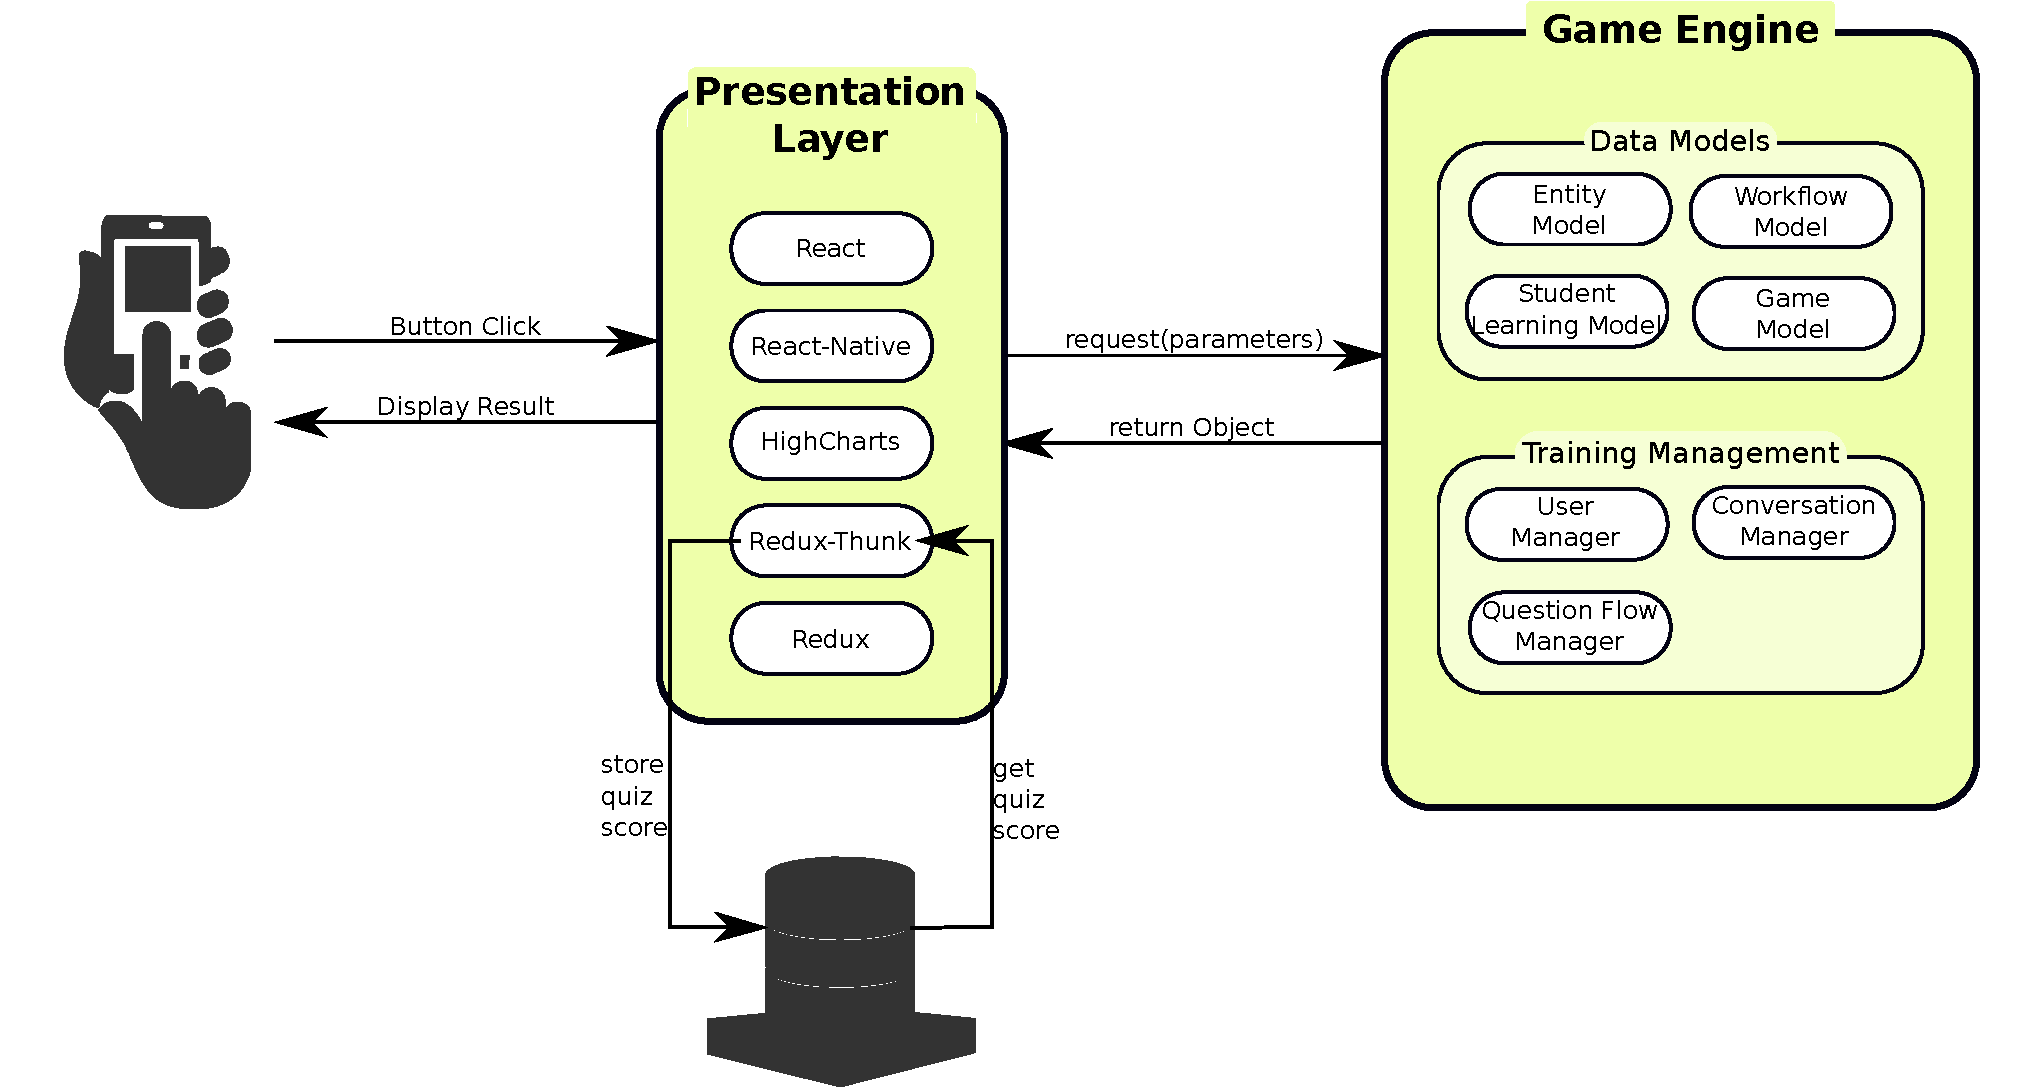
\includegraphics[scale=0.4]{Architecture}
	\caption {Overview of the system architecture}
	\label{fig:Architecture}
\end{figure}

\subsection{Presentation Layer}
The presentation layer is what the user sees and interacts with when using the application. React Native \parencite{ReactNative} is a JavaScript framework, used to build cross platform mobile applications for Android, iPhone and UWP. It is based on React \parencite{React}, where it uses React components to build user interfaces for mobile applications. 

For managing the state of the application, we use another JavaScript framework, Redux \parencite{Redux}. It is sort of a repository of functions and variables. When the student clicks on a button in the application, it will trigger a function in the Redux repository. The function can send a request to the Game Engine or do some calculations in its own. Then update a variable in the repository which is connected to a variable in the React Component, and the result is shown on the student's phone.

As the Redux repository is synchronous, we need the framework Redux-Thunk \parencite{ReduxJS-thunk} to make asynchronous calls. A student's scores for a quiz is stored in the database on the student's phone. The game engine uses the scores to find questions at the right difficulty level for the student. As database calls are asynchronous, we need Redux-Thunk to make functions which can do asynchronous communication between Redux and the database. 

HighCharts \parencite{Highsoft} is a JavaScript framework used for making interactive charts. We use it to visualizing how well the user performed, and how far he is from advancing to more difficult questions.  

\subsection{Game Engine} 
The game engine initializes the quiz, controls the training flow, produces questions with answering elements and keeps track of the user's performance. 

The data models are used to hold information and represent a domain of concepts. The entity model represents a patient at different stages under a clinical encounter. The workflow model describes different processes at a clinical encounter. The game model holds relevant game information such as questions at different categories and difficulty levels, distractions, points and penalties for each distraction, answer keys and answer key explanations. The student learning model keeps track of the student's scores at different quizzes.

The managers are conceptual, used to better describe the responsibilities of the game engine in this section. 

The question flow manager adapts the questions to the knowledge level of the student, and is flexible such that the student can choose his own path through the completion of each difficulty level. 

The conversation manager puts the questions with belonging answer elements in a sequence such that they fit to a scenario, using the workflow model. The conversation manager produces questions and answer keys from a template, in which the entity model is used to fill in data for the place holders in the template.

The user manager keeps track of the user's skill, based on the performance on previous quizzes. The scores on the current quiz, and it measures the user's progression. 
